\documentclass[a4paper,14pt]{article}

\usepackage{comment} % Para comentar várias linhas ao mesmo tempo

%matemática
\usepackage{amsmath}
\usepackage{amssymb}

%diagramação
\usepackage{extsizes}
\everymath{\displaystyle}
\usepackage{geometry}
\usepackage{fancyhdr}
\usepackage{multicol}
\usepackage{graphicx}
\usepackage[brazil]{babel}
\usepackage[shortlabels]{enumitem}
\usepackage{cancel}
\usepackage{textcomp}
\usepackage{tcolorbox}

%tabelas
\usepackage{array} % Para melhor formatação de tabelas
\usepackage{longtable}
\usepackage{booktabs}  % Para linhas horizontais mais bonitas
\usepackage{float}   % Para usar o modificador [H]
\usepackage{caption} % Para usar legendas em tabelas
\usepackage{wrapfig} % Para usar tabelas e figuras flutuantes


%tikzpicture
\usepackage{tikz}
\usepackage{scalerel}
\usepackage{pict2e}
\usepackage{tkz-euclide}
\usetikzlibrary{calc}
\usetikzlibrary{patterns,arrows.meta}
\usetikzlibrary{shadows}
\usetikzlibrary{external}

%pgfplots
\usepackage{pgfplots}
\pgfplotsset{compat=newest}
\usepgfplotslibrary{statistics}
\usepgfplotslibrary{fillbetween}

%colours
\usepackage{xcolor}



\columnsep=2cm
\hoffset=0cm
\textwidth=8cm
\setlength{\columnseprule}{.1pt}
\setlength{\columnsep}{2cm}
\renewcommand{\headrulewidth}{0pt}
\geometry{top=1in, bottom=1in, left=0.7in, right=0.5in}

\pagestyle{fancy}
\fancyhf{}
\fancyfoot[C]{\thepage}

\begin{document}
	
	\noindent\textbf{6FMA82 - Matemática} 
	
	\begin{center}Escrevendo produtos como potências (Versão estudante)
	\end{center}
	
	\noindent\textbf{Nome:} \underline{\hspace{10cm}}
	\noindent\textbf{Data:} \underline{\hspace{4cm}}
	
	%\section*{Questões de Matemática}
	
	\begin{multicols}{2}
		\noindent Na multiplicação $a \cdot b = c$, dizemos que $a$ e $b$ são os fatores e $c$ é o produto. \\
		Quando os fatores forem todos iguais, podemos escrever a multiplicação na forma de potência. \\
		Por exemplo, em vez de $2 \cdot 2 \cdot 2$, podemos escrever $2^3$. Nesse caso, dizemos que 2 é a base da potência e 3 é o expoente da potência.
		\begin{center}
			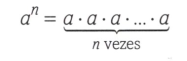
\includegraphics[width=0.7\linewidth]{6FMA82_imagens/imagem1}
		\end{center}
		\noindent\textsubscript{-----------------------------------------------------------------------}
		\begin{enumerate}
			\item Escreva na forma de potência os seguintes produtos.
			\begin{enumerate}[a)]
				\item $(-5)(-5)(-5)(-5)(-5)$ \\\\\\\\\\\\
				\item $6 \cdot 6 \cdot 6 \cdot 6$ \\\\\\\\\\\\
				\item $0 \cdot 0 \cdot 0 \cdot 0$ \\\\
				\item $3^2 \cdot 3^2 \cdot 3^2 \cdot 3^2 \cdot 3^2 \cdot 3^2$ \\\\\\\\\\\\
				\item $14 \cdot 14 \cdot 14$ \\\\\\\\\\\\
				\item $21 \cdot 21 \cdot 21 \cdot ... \cdot 21$ (88 termos)
			\end{enumerate}
			\item Efetue.
			\begin{enumerate}[a)]
				\item $(-5)^0$ \\\\\\\\\\
				\item $(-7)^2$ \\\\\\\\\\
				\item $(-5)^3$ \\\\\\
				\item $2^-5$ \\\\\\\\\\
				\item $(-2)^{-3}$ \\\\\\\\\\
				\item $\bigg(\frac{4}{9}\bigg)^{-2}$ \\\\\\\\\\
				\item $\bigg(-\frac{1}{4}\bigg)^{-4}$ \\\\\\\\\\
			\end{enumerate}
			\item Efetue.
			\begin{enumerate}[a)]
				\item $-4^3$ \\\\\\\\\\
				\item $(-4)^3$ \\\\\\\\\\
				\item $-(-4)^3$ \\\\\\\\\\
				\item $-\bigg(-\frac{1}{5}\bigg)^{-2}$ \\\\\\\\\\
				\item $-\bigg(-\frac{5}{3})^{-3}$ \\\\\\\\\\
				\item $\bigg(\frac{1}{9}\bigg)^{-2}-\bigg(\frac{1}{4}\bigg)^{-3}$ \\\\\\\\\\
				\item $-4^2 -6^2$ \\\\\\\\\\
			\end{enumerate}
			\item Se $x$ é inteiro e $x \neq 0$, então $x^2$ é sempre um número positivo e $-x^2$ é sempre um número negativo. Diga, das expressões abaixo, quais geram sempre números positivos e quais geram sempre números negativos, sabendo que $x \in \mathbb{Z}$ e $x \neq 0$.
			\begin{enumerate}[a)]
				\item $x^2$ \\\\\\
				\item $x^3$ \\\\\\
				\item $-x^2$ \\\\\\
				\item $x^4$ \\\\\\
				\item $(-x)^2$ \\\\\\
				\item $-x$ \\\\\\
				\item $x$ \\\\\\
				\item $(-x)^3$ \\\\\\
				\item $(-x)^4$ \\\\\\
				\item $(-x)^{42}$ \\\\\\
				\item $x^{37}$ \\\\\\
				\item $x^{24}$ \\\\\\
			\end{enumerate}
			\textbf{Desafio olímpico} \\\\
			(OBMEP) Podemos colocar de várias maneiras um par de parênteses na expressão $20 : 2 + 3 \cdot 6$ e $20 : (2 + 3 \cdot 6)$. Qual é o maior valor que se pode obter desse modo?
			\begin{enumerate}[a)]
				\item 24
				\item 28
				\item 30
				\item 78
				\item 138
			\end{enumerate}
			\item Escreva na forma de potência os seguintes produtos:
			\begin{enumerate}[a)]
				\item $(-4)(-4)(-4)(-4)(-4)(-4)$
				\item $7 \cdot 7 \cdot 7 \cdot 7 \cdot 7 \cdot 7 \cdot 7 \cdot 7$
				\item $2^3 \cdot 2^3 \cdot 2^3 \cdot 2^3 \cdot 2^3$
				\item $19 \cdot 19 \cdot 19 \cdot 19$
				\item $0 \cdot 0 \cdot 0 \cdot 0 \cdot 0 \cdot 0 \cdot 0$
				\item $1 \cdot 1 \cdot 1 \cdot 1 \cdot 1 \cdot 1 \cdot 1 \cdot 1 \cdot 1 \cdot 1$
				\item $(-6) \cdot (-6) \cdot ... \cdot (-6)$  (12 termos)
				\item $52 \cdot 52 \cdot ... \cdot 52$ (99 termos)
			\end{enumerate}
			\item Efetue.
			\begin{enumerate}[a)]
				\item $(-8)^0$
				\item $(-3)^2$
				\item $4^3$
				\item $(-3)^4$
				\item $6^2$
				\item $(-2)^3$
				\item $(-1)^9$
				\item $(-1 001)^0$
				\item $(-5)^{-3}$
				\item $-(8)^{-2}$
				\item $2^9$
				\item $(-2)^9$
				\item $8^0$
				\item $\bigg(\frac{2}{5}\bigg)^{-4}$
				\item $\bigg(-\frac{9}{5}\bigg)^{-2}$
				\item $48^1$
				\item $(13)^{-2}$
				\item $(-4)^3$
				\item $(-48)^{-1}$
				\item $0^{99}$
				\item $-3^3$
				\item $(-3)^3$
				\item $-(-9)^2$
				\item $-\bigg(-\frac{1}{7}\bigg)^{-3}$
				\item $-(-6)^3$
				\item $-\bigg(\frac{7}{6}\bigg)^{-2}$				
			\end{enumerate}
			\begin{enumerate}[A)]
				\item $-4^4-3^5$ \\\\\\\\
				\item $(-2)^{-4}-(-4)^{-2}$ \\\\\\\\
				\item $-(-4^4 + 3^5)$ \\\\\\\\
				\item $(-5)^2 - 6^2$ \\\\\\\\
				\item $-\bigg(-\frac{1}{5}\bigg)^{-2} + \bigg(\frac{1}{2}\bigg)^{-4}$ \\\\\\\\
				\item $-4^2 + 3^2 -(-2)^3$ \\\\\\\\
				\item $-(-4)^3-(-3)^4+(-5)^0$ \\\\\\\\
				\item $-21^0 + 5^3 -(-3)^3 - 1^8$ \\\\
				\item $-(7)^0 -(-8)^2 + (-6)^2 -(-1)^0$ \\\\\\\\
			\end{enumerate}
			\item Se $x$ é inteiro e $x \neq 0$, então $x^2$ é sempre um número positivo e $-x^2$ é sempre um número negativo. Diga quais das expressões abaixo geram sempre números positivos e quais geram sempre números negativos, sabendo que $x \in \mathbb{Z}$ e $x \neq 0$.
			\begin{enumerate}[a)]
				\item $-x$
				\item $x^3$
				\item $x^2$
				\item $-x^2$
				\item $x^6$
				\item $(-x)^2$
				\item $-x^3$
				\item $x$
				\item $(-x)^3$
				\item $x^45$
				\item $(-x)^8$
				\item $(-x)^{1000}$
			\end{enumerate}
			\item Se $x \in \mathbb{Z}$, então $x^2 \geq 0$. Logo $x^2 + 1 > 0$ para todo inteiro $x$. Diga, das expressões a seguir, quais geram sempre números positivos e quais geram sempre números negativos, sabendo que $x \in \mathbb{Z}$
			\begin{enumerate}[a)]
				\item $x^2 + 6$
				\item $x^2 -1$
				\item $x^6 + 3$
				\item $(x + 1)^2$
				\item $(x^2 + 1)^2$
				\item $x^3 + 1$
				\item $-x^2 - 5$
				\item $x^7 + 2$
				\item $x^8 + 4$
			\end{enumerate}
			\item Um professor escreveu o seguinte problema na lousa: "Qual o valor da potência cujo expoente é a soma de parcelas -3 e 8, e sua base é uma diferença, na qual o minuendo é a potência de base -2 e expoente 7 e o subtraendo é a potência de base -5 e expoente 3?"
			Um aluno resolveu da seguinte maneira em seu caderno:
			$((-5)^3)-(-2)^7)^{(-3 + 8)}$ \\
			$= (125 - 128)^5$ \\
			$=(-3)^5$ \\
			$= 243$ \\
			O professor informou que a resposta final era -243.
			\begin{enumerate}[a)]
				\item Quais foram os erros cometidos pelo aluno? Indique-os. \\\\\\\\\\\\
				\item Resolva a expressão corretamente. \\\\\\\\\\\\
			\end{enumerate}
		\end{enumerate}
	\end{multicols}
\end{document}